\begin{progprob}
    Suppose we are given a weighted, undirected graph $G = (V, E, \omega)$ in
    which the edge weights represent \emph{similarity}; for example, the
    similarity between two users in a social network. Given a number $\lambda$,
    we will say that the \emph{clusters} of $G$ are the connected components of
    the graph after all edges whose weight is less than $\lambda$ have been
    removed. There are other ways of defining the clusters of a weighted graph,
    but this is one natural way.

    In \python{cluster.py}, write a function \python{cluster(graph, weights,
    level)} which computes the clusters of a weighted graph. Here,
    \python{graph} is an instance of \python{dsc40graph.UndirectedGraph},
    \python{weights(u, v)} is a function returning the weight of edge $(u, v)$,
    and \python{level} is a number representing the level at which to find the
    clusters. Its return value should be a \python{frozenset}\footnote{
        We use \python{frozenset}s here because clusters are sets, but \python{set}s
        cannot be elements within other \python{set}s since they are not hashable.
    }
    containing \python{frozenset}s;
    the inner \python{frozenset}s should contain the nodes in a cluster.

    Your code should not modify the graph in any way and it should not create a copy
    of the graph. It should run in $\Theta(V + E)$ time.

    Note that \python{weights} is a function that will be constructed by us and
    passed to your function; you will not need to create it (except in your own
    tests).

    For example, given the following graph:

    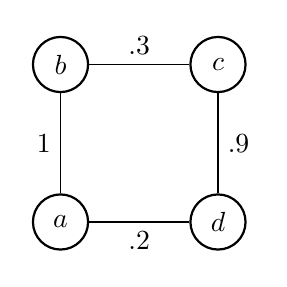
\begin{tikzpicture}
        \tikzset{n/.style={draw, circle, thick, inner sep=0em, minimum width=.7cm}}
        \draw node[n] (a) at (0,0) {$a$};
        \draw node[n] (b) at (0,2) {$b$};
        \draw node[n] (d) at (2,0) {$d$};
        \draw node[n] (c) at (2,2) {$c$};

        \draw (a) edge node[left] {1} (b);
        \draw (c) edge node[right] {.9} (d);
        \draw (a) edge node[below] {.2} (d);
        \draw (b) edge node[above] {.3} (c);
    \end{tikzpicture}

    The output when run with a level of 0.4 should be:

    \begin{minted}[autogobble]{python}
        >>> def weights(x, y):
        ... x, y = (x, y) if x < y else (y, x)
        ... return {("a", "b"): 1, ("b", "c"): .3, ("c", "d"): .9, ("a", "d"): .2}[(x, y)]
        >>> cluster.cluster(graph, weights, 0.4)
        frozenset([frozenset(['a', 'b']), frozenset(['c', 'd'])])
    \end{minted}

    Note: you might see curly braces instead of square brackets in the output -- that's OK.
    Different versions of Python print frozensets differently.

    \begin{soln}
        For this problem, we can use a modified BFS or DFS (solution
        is BFS) to find the connected components or clusters while
        ignoring edges that are below the weight threshold. Returning
        elements visited is important as scanning the status array
        for changes can lead to a higher runtime of $\Theta(V^2 + E)$
        This approach takes $\Theta(V + E)$ time in total.

        \inputminted{python}{\thisdir/include-solution/cluster.py}
   \end{soln}

\end{progprob}
